\chapter{Diseño del agente}

En este capítulo se detallará el diseño del agente propuesto para la resolución del problema. 

Se empezará presentando la formalización del conocimiento usada (estado, acción y recompensa) y las características físicas del agente. Tras esto, se describirán las dos arquitecturas propuestas para el agente: una primera basada en una red neuronal convolucional, y una segunda basada en una red profunda híbrida. Finalmente, se explicará el proceso de actuación y entrenamiento del agente.

\section{Caracterización del conocimiento}

En esta sección se describe la caracterización del conocimiento realizada, centrándose en los puntos principales del aprendizaje por refuerzo: el \textbf{estado}, las \textbf{acciones} disponibles y las \textbf{recompensas} que recibe el agente.

\subsection{Estado}

El \textbf{estado} (la percepción que tiene el agente del entorno) consta de tres elementos:

\begin{itemize}
	\item \textbf{Imagen de profundidad:} Una imagen en escala de grises representando las observaciones de la cámara de profundidad. Esta imagen tiene un tamaño de $(256 x 256)$ píxeles, con los valores de cada celda en el rango $[0.0, 1.0]$ (donde $0.0$ o negro significa cercanía a la cámara y $1.0$ o blanco significa lejanía). Se puede ver un ejemplo de la imagen en la Figura \ref{fig:chap5-estado}.
	
	Se ha optado por añadir este valor por el planteamiento del problema. Al buscar diseñar un agente reactivo frente a obstáculos, es importante que el agente sea capaz de percibir cualquier objeto que se encuentre en su camino. Una cámara de profundidad nos permite estimar las distancias a estos obstáculos de forma rápida y simple.	
	
\begin{figure}[h]
    \centering
    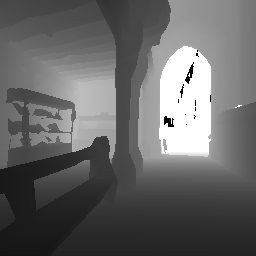
\includegraphics{imagenes/cap5/normalized.png}
    \caption{Ejemplo de imagen de profundidad usada como parte del estado.}
    \label{fig:chap5-estado}
\end{figure}			
		
	\item \textbf{Distancia a la meta:} Un valor decimal que representa la distancia actual entre el agente y la meta en metros.
	
	Este valor forma parte del estado al ser parte del cálculo de la recompensa (como se verá posteriormente). Además, es importante que el agente sea capaz de estimar la distancia hasta la meta para que tenga la posibilidad de aprender cuando detenerse.
	
	\item \textbf{Ángulo respecto a la meta:} Un valor decimal que representa el ángulo que debería girar el agente para enfocarse hacia la meta, en radianes. Un valor positivo significa que el agente debería girar hacia la derecha, mientras que un valor negativo significa que el agente debería girar hacia la izquierda.
	
	Si bien este valor no forma parte del cómputo de la recompensa, se ha optado por añadir el ángulo al estado para permitir al agente tener la posibilidad de aprender información respecto a su orientación que no podría aprender en otro caso.
\end{itemize}

Si bien se consideró añadir una \textbf{imagen en color} al estado, finalmente se ha optado por no incluirla. Esto se debe a que la información que añade resulta superflua, ya que la cámara de profundidad incluye toda la información necesaria para el cálculo de obstáculos. Además, los escenarios de interior son complejos con altos niveles de ruido, por lo que una cámara de color podría llevar a sobreajustes (al aprender el aspecto de los interiores frente a los obstáculos).

Un estado se considera \textbf{final} cuando el agente lo finaliza (ya sea por realizar la acción especifica de terminar o por superar el número máximo de acciones permitidas). Este estado final puede ser \textbf{exitoso} si la distancia a la meta es menor a un umbral (por defecto $0.3$ metros), o \textbf{fallido} en otro caso.

\subsection{Acciones}

El agente es capaz de realizar \textbf{cuatro} acciones en total:

\begin{itemize}
	\item \textbf{Desplazarse} hacia delante. Por defecto, el desplazamiento es de $0.25$ metros.
	\item \textbf{Girar} hacia la derecha o la izquierda. Por defecto, el giro es de $10$ grados.
	\item \textbf{Finalizar el episodio}. La inclusión de una acción para finalizar el episodio es una de las principales sugerencias de Peter Anderson \textit{et al.} \cite{DBLP:journals/corr/abs-1807-06757} para la evaluación de agentes físicos.
\end{itemize}

Como se comentó en el Capítulo 2 y se puede observar, el agente no es capaz de un movimiento omnidireccional (como sí podría un dron volador). El agente únicamente puede desplazarse hacia adelante, necesitando rotar sobre si mismo para cambiar la dirección de su movimiento.

\subsection{Recompensas}

El sistema de recompensas diseñado está basado en el sistema originalmente propuesto por Carlos Sampedro \textit{et al.} \cite{Sampedro2018}, siendo éste un sistema de recompensas basado en campos de potenciales artificiales, con un \textbf{atractor} que atrae al agente hacia la meta y \textbf{repulsores} que repelen al agente de los obstáculos. Ahora bien, este sistema ha sido adaptado a la arquitectura del agente desarrollado (con cámara de profundidad), y se han propuesto variantes para evaluar su rendimiento.

El cálculo de la recompensa de un estado se puede dividir en los siguientes pasos:
\begin{enumerate}
	\item Preprocesamiento de la imagen del estado.
	\item Identificación de obstáculos en la imagen (con dos posibles métodos)
	\item Cálculo de los potenciales atractivos y repulsivos.
	\item Cálculo de la recompensa final (con dos posibles métodos)
\end{enumerate}

Estos pasos se describirán a continuación.

\subsubsection{Preprocesamiento de la imagen de profundidad}

Para calcular las recompensas posteriormente, es necesario identificar los obstáculos o los objetos que pueden suponer un riesgo en la imagen. Ahora bien, no se puede usar la imagen directamente al contener ruido e información necesaria. Por esto, se realiza un preprocesamiento antes de identificar los obstáculos en la imagen, siguiendo los siguientes pasos:

\begin{enumerate}
	\item \textbf{Normalización:} Por defecto, la imagen obtenida por la cámara está formada por valores decimales en el rango $[0.0, 1.0]$. Ahora bien, para poder trabajar por la imagen es necesario que estos valores sean enteros en el rango $[0, 255]$ por compatibilidad con otras librerías. Por tanto, se transforman los valores de un rango al otro.
	\item \textbf{Recorte de los extremos:} Se ha visto que los extremos superiores e inferiores de la imagen (el suelo y el techo) no aportan información útil a la hora de calcular la recompensa, pudiendo llegar a introducir ruido y obstáculos que no existen.
	
	Para evitar esto, se recortan los extremos superiores e inferiores de la imagen. Por defecto, se recortan $35$ pixeles de cada extremo. Este valor se ha obtenido de forma empírica con pruebas y es heurístico.
	\item \textbf{Eliminación de artefactos del simulador:} En ocasiones, el simulador introduce ruido en la imagen en forma de partes de color negro puro (con valor $0$). Estos artefactos no son reales (al no ser capaz la cámara de devolver un valor tan bajo en la práctica) y pueden interferir con la detección de obstáculos, por lo que es necesario eliminarlos.
	
	Para eliminarlos, se sustituyen todos los valores de $0$ (negro puro) por $255$ (blanco puro). Esto hará que sean ignorados en los pasos posteriores.
	
	\item \textbf{Umbralización (\textit{Thresholding}):} Es necesario identificar los obstáculos en la imagen. Si bien se podría haber optado por alguna técnica de búsqueda de contornos (como \textit{Canny}), se ha optado por realizar una umbralización, donde todos los valores de la imagen son reemplazados usando la siguiente fórmula:
	\[
		imagen(x) = 
		\begin{cases}
			1,& \text{si } imagen(x) \leq suelo(255*umbral)\\
			0,& \text{en cualquier otro caso} 
		\end{cases}
	\] 
	Donde $umbral$ es el valor que se ha tomado para umbralización en el rango $[0.0, 1.0]$ (siendo por defecto $0.15$, elegido de forma empírica).
	
	En esencia, esta fórmula sustituye todos los valores menores a $suelo(255*umbral)$ (cercanos a la cámara) por $1$ (blanco), mientras que el resto de valores (lejanos) son sustituidos por $0$. De esta forma, se obtiene una imagen binaria en la que solo se conservan los obstáculos más cercanos.
	
	\item \textbf{Eliminación de ruido:} El proceso de umbralización puede crear ruido, como pueden ser regiones negras pequeñas dentro de contornos blancos más grandes, que pueden afectar al rendimiento.
	
	Para eliminar este ruido, se usa una técnica de \textit{apertura morfológica}, que consiste en una dilatación (aumentar el volumen de los objetos en la imagen) seguida de una erosión (disminuir el volumen de los objetos en la imagen). Esto reduce el ruido incluido dentro de los contornos, sin afectar demasiado al volumen final.
	
	\item \textbf{Dilatación:} El paso final consiste en dilatar (aumentar el volumen) de la imagen, para evitar perdidas de información provocadas por la eliminación de ruido del paso previo. Esta dilatación final no afectará al proceso de identificación de obstáculos por su funcionamiento, que se verá posteriormente.
\end{enumerate}

Se puede observar un ejemplo de este proceso en la Figura \ref{fig:chap5-imageprocess}.

\begin{figure*}
    \centering
    \begin{subfigure}[b]{.475\textwidth}
    \centering
    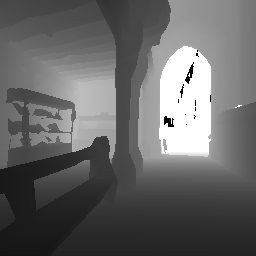
\includegraphics[width=\textwidth]{imagenes/cap5/normalized.png}
    \caption{Imagen normalizada.}
    \end{subfigure}
    \begin{subfigure}[b]{.475\textwidth}
    \centering
    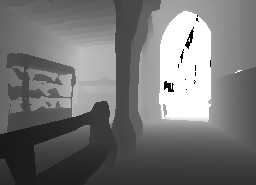
\includegraphics[width=\textwidth]{imagenes/cap5/trimmed.png}
    \caption{Imagen recortada.}
    \end{subfigure}
    
    \begin{subfigure}[b]{.475\textwidth}
    \centering
    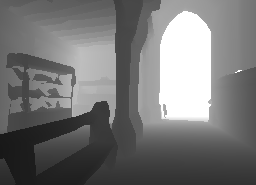
\includegraphics[width=\textwidth]{imagenes/cap5/filled.png}
    \caption{Imagen sin artefactos.}
    \end{subfigure}
    \begin{subfigure}[b]{.475\textwidth}
    \centering
    
\includegraphics[width=\textwidth]{imagenes/cap5/thresholded.png}
    \caption{Imagen con umbral aplicado.}
    \end{subfigure}

	\begin{subfigure}[b]{.475\textwidth}
    \centering
    
\includegraphics[width=\textwidth]{imagenes/cap5/cleaned.png}
    \caption{Imagen sin ruido.}
    \end{subfigure}
    \begin{subfigure}[b]{.475\textwidth}
    \centering
    
\includegraphics[width=\textwidth]{imagenes/cap5/dilated.png}
    \caption{Imagen dilatada.}
    \end{subfigure}

    \caption{Procesamiento realizado sobre la imagen de profundidad.}
    \label{fig:chap5-imageprocess}
\end{figure*}

\subsubsection{Identificación de los obstáculos y la distancia en la imagen}

Tras el preprocesamiento de la imagen, es necesario identificar los obstáculos en la imagen   y estimar la distancia a la que éstos se encuentran. Para eso, se han propuesto dos métodos:

\begin{itemize}
	\item \textbf{Método de contornos:} Este método se basa en la propuesta original de Carlos Sampedro \textit{et al.} \cite{Sampedro2018}. 
	
	La idea principal del método es identificar los contornos que tengan un área mínimo (experimentalmente determinado como $250$ pixeles) en la imagen preprocesada. A partir de estos contornos, se crean máscaras en la imagen original para extraer los obstáculos de nuevo en escala de grises. Finalmente, se obtiene la cercanía de esos obstáculos (a partir del pixel de valor mínimo), usando la siguiente estimación:
	\[distancia = \frac{(pixel\_min / 256) * distancia\_estimada}{umbral\_obstaculo}\]
Donde $pixel\_min$ es el pixel de menor valor en el obstáculo (en el rango ${0, 255}$), $distancia\_estimada$ es un valor heurístico que indica la distancia a la que se encontraría un obstáculo en el umbral (estimado como $2$ metros) y $umbral\_obstaculo$ es el umbral que se ha usado durante la umbralización ($0.15$).

Se puede ver el pseudocódigo del proceso en la Figura \ref{alg:contour}.

\begin{figure}[h]
\begin{algorithm}[H]
\SetAlgorithmName{Algoritmo}{algoritmo}{Lista de algoritmos}
\caption{Identificación de distancias con método de contornos}
\textbf{Variables:} Imagen preprocesada $imagen\_p$, imagen recortada $imagen\_r$, umbral usado durante preprocesamiento $umbral$, distancia estimada hasta el umbral en metros $dist$, área mínima de los contornos en píxeles $area\_min$.\\
\textbf{1.} Inicializa una lista para almacenar las distancias obtenidas, $distancias$.\\
\textbf{2.} Extrae los contornos de la imagen $imagen\_p$ a una lista $contornos$.\\
\textbf{3.} Para cada contorno $cont$ de area $area\_contorno$ en $contornos$, con $area\_contorno \geq area\_min$:\\
\Indp \textbf{3.1.} Aplica una máscara con la forma de $cont$ a $imagen\_r$, obteniendo el obstáculo $obs$ (el obstáculo tal y como está representando en la imágen $imagen\_r$, en escala de grises).\\
\textbf{3.2.} Obtén la distancia mínima en $obs$ (el valor mínimo), $dist\_obs$.\\
\textbf{3.3.} Convierte $dist\_obs$ de un valor entero en el rango $\{0, 255\}$ a una distancia en metros mediante una equivalencia usando $umbral$ y $dist$.\\
\textbf{3.4.} Si $dist\_obs \leq dist$, almacena $dist\_obs$ en $distancias$.\\
\Indm \textbf{4.} Devuelve $distancias$.
\end{algorithm}
\hrule
\caption{Pseudocódigo del método de contornos para identificar distancias a obstáculos.}
\label{alg:contour}
\end{figure}
	
	\item \textbf{Método de columnas:} Un método original, consistente en dividir la imagen  en columnas de misma anchura, siendo cada columna un posible obstáculo. 
	
	El método consiste en dividir la imagen preprocesada en $8$ (elegido experimentalmente) columnas de anchura idéntica. Tras esto, se cuenta el número de píxeles blancos (obstáculos) en cada columna, considerando las columnas que tengan una cantidad superior al área mínima ($250$ píxeles como se ha mencionado previamente) como obstáculos. Para estas columnas, se estima la distancia a partir de una columna equivalente de la imagen original, usando la fórmula descrita previamente:
	\[distancia = \frac{(pixel\_min / 256) * distancia\_estimada}{umbral\_obstaculo}\]
Donde $pixel\_min$ es el pixel de menor valor en el obstáculo (en el rango ${0, 255}$), $distancia\_estimada$ es un valor heurístico que indica la distancia a la que se encontraría un obstáculo en el umbral (estimado como $2$ metros) y $umbral\_obstaculo$ es el umbral que se ha usado durante la umbralización ($0.15$).

Se puede ver el pseudocódigo del proceso en la Figura \ref{alg:column}.

\begin{figure}[h]
\begin{algorithm}[H]
\SetAlgorithmName{Algoritmo}{algoritmo}{Lista de algoritmos}
\caption{Identificación de distancias con método de columnas}
\textbf{Variables:} Imagen preprocesada $imagen\_p$, imagen recortada $imagen\_r$, umbral usado durante preprocesamiento $umbral$, distancia estimada hasta el umbral en metros $dist$, área mínima de los contornos en píxeles $area\_min$.\\
\textbf{1.} Divide las imágenes $imagen\_p$ y $imagen\_r$ en columnas de anchuras iguales, $columnas\_p$ y $columnas\_r$.\\
\textbf{2.} Para cada columna $col$ con $pixeles$ pixeles blancos en $columnas\_p$ y $col\_r$ en $columnas\_r$, cumpliendo que $pixeles \geq area\_min$:\\
\Indp\textbf{2.1.} Obtén la distancia mínima en $col\_r$ (el valor mínimo), $dist\_obs$.\\
\textbf{2.2.} Convierte $dist\_obs$ de un valor entero en el rango $\{0, 255\}$ a una distancia en metros mediante una equivalencia usando $umbral$ y $dist$.\\
\textbf{2.3.} Si $dist\_obs \leq dist$, almacena $dist\_obs$ en $distancias$.\\
\Indm \textbf{3.} Devuelve $distancias$.
\end{algorithm}
\hrule
\caption{Pseudocódigo del método de columnas para identificar distancias a obstáculos.}
\label{alg:column}
\end{figure}

Este método se propone al considerar que el método anterior daría la misma importancia a un obstáculo grande (que ocupa gran parte de la pantalla) y a uno pequeño siempre y cuando estuviesen a la misma distancia. La idea es remediar ese problema, dando más peso a los obstáculos más grandes. Además, al evitar tener que usar algoritmos de búsqueda de contornos, se espera que la velocidad de ejecución sea mayor.

\end{itemize}

\subsubsection{Cálculo del potencial atractivo y repulsivo}

Tras el cálculo de las distancias a los obstáculos, se calcula el valor de los potenciales atractivos y repulsivos. Este cálculo es equivalente al propuesto por Carlos Sampedro \textit{et al.} \cite{Sampedro2018} originalmente.

El \textbf{potencial atractivo} es la fuerza con la que la meta atrae al agente. Cuanto más cerca esté el agente de la meta, mayor debe ser su influencia. Este potencial se obtiene con la siguiente fórmula:
\[U_{atr} = \alpha p_{goal}(t_r)\]
Donde $\alpha$ es una ganancia positiva usada para aumentar la influencia del potencial (estimada empíricamente como $100$) y $p_{goal}(t_r)$ es la distancia euclídea entre la posición actual del agente y la meta.

El \textbf{potencial repulsivo} es la suma de las fuerzas con las que los obstáculos repelen al agente. Cuantos más obstáculos perciba el agente y más cerca se encuentren, mayor debe ser su influencia. Este potencial se obtiene con la siguiente fórmula:
\[U_{rep} = \beta \sum_{i=1}^{N}(\frac{1}{k+l_i}-\frac{1}{k+l_{max}})\]
Donde $N$ es el número total de obstáculos detectados, $k$ es una constante usada para limitar la influencia de los obstáculos (con valor por defecto $0.04$), $l_i$ es la distancia al obstáculo $i$ en metros, $l_{max}$ es la distancia máxima a la que se detectan los obstáculos (con valor por defecto $2$ metros) y $\beta$ se obtiene con la siguiente fórmula:
\[
\beta = 
\begin{cases}
\delta,& \text{si } p_{goal}(t_r) > d_{infl}\\
\frac{\delta}{exp[4(d_{infl}-p_{goal}]},& \text{si } p_{goal}(t_r) \leq d_{infl}
\end{cases}
\]
Donde $\delta$ es una ganancia positiva usada para aumentar la influencia del potencial (estimada empíricamente como $15$) y $d_{infl}=0.75 l_{max}$ es una distancia a partir de la cual la influencia del potencial repulsivo se disminuye, para fomentar al agente a acercarse a la meta cuando se encuentra próximo a ésta.

Tras el cálculo de ambos potenciales, es posible calcular el \textbf{valor del estado actual}. Cuanto mayor es el valor del estado, mejor estado se considera que es. Este valor se comparará con el valor del estado previo para comprobar si ha mejorado o empeorado, y obtener una recompensa a partir de ello.

Este valor se calcula como:
\[valor_t=-U_{atr}-U_{rep}\]

\subsubsection{Cálculo de la recompensa final}
 
Tras haber calculado los potenciales y el valor del estado, es posible obtener la recompensa final a partir de las siguientes reglas:

\begin{itemize}

\item Si el episodio ha finalizado (ya sea por la acción correspondiente o por limite de acciones) y el agente no está en rango de la meta: \textbf{-100}.

La penalización por finalizar un episodio sin exito es muy alta para evitar que el agente finalice el episodio antes de tiempo con la intención de evitar penalizaciones por sus acciones.

\item Si el episodio ha finalizado (ya sea por la acción correspondiente o por limite de acciones) y el agente está en rango de la meta: \textbf{+10}.

La recompensa por finalizar un episodio con éxito es menor, pero sigue siendo elevada para fomentar al agente a llegar a la meta y finalizar en ella.

\item En cualquier otro caso:

Si el episodio no ha finalizado tras la acción del agente, se procede a calcular la recompensa a partir de los valores del estado actual y el previo:
\[recompensa = (valor_t - valor_{t-1}) - 0.25, \text{acotado en el rango } [-100, +10]\]

Si el valor del estado alcanzado tras realizar la acción es mayor (la acción lleva a un estado mejor) la recompensa será positiva, mientras que si el valor es menor (la acción lleva a un estado peor) la recompensa será negativa. De esta forma, se fomenta que el agente intente mejorar su posición continuamente.

El término $-0.25$ es una penalización por paso, usada para evitar que el agente permanezca en bucles infinitos sin recompensa y acelerando su progreso.

\end{itemize} 

Una alternativa propuesta es incluir una regla adicional al cálculo de recompensas:
\begin{itemize}
	\item Si el agente ha colisionado con algún obstáculo tras la acción: \textbf{-100} y \textbf{finaliza el episodio}.
	
	Con esta regla adicional, se penaliza notablemente que el agente colisione con los obstáculos, fomentando que evite cualquier colisión con el entorno. Estas colisiones se comprueban usando la métrica \textit{COLLISIONS}.
\end{itemize}

\section{Características físicas del agente}

[NO SE SI DEJAR ESTE PUNTO? SERIA PRINCIPALMENTE HABLAR DE LOS SENSORES INCLUIDOS Y DE QUE NO PUEDE ANDAR... PERO ESO SE INTUYE A PARTIR DE LA DEFINICION DEL ESTADO NO?]

\section{Arquitectura del agente}

\subsection{Propuesta 1: Red convolucional (CNN)}

\subsection{Propuesta 2: Red híbrida (CNN + MLP)}

\section{Actuación del agente}
[exploracion explotacion]

\section{Entrenamiento del agente}

\subsection{\textit{Experience Replay}}

\subsection{Memorización de experiencias}

\subsection{Aprendizaje a partir de las experiencias}

\subsection{Documentación del entrenamiento}